\documentclass[ngerman,english]{ijsra}



\def\IJSRAidentifier{\currfilebase}%<<<< DO NOT change this line
\def\shorttitle{IARSS 2016 Review}
\def\maintitle{Review: Iron Age Research Student Symposium 2016}
\def\shortauthor{Sarah Scheffler, Andy Lamb, Rachel Wilkinson}
\def\authormail{iarss2016@gmail.com}
\def\affiliation{University of Leicester}
%\def\thanknote{}
\def\keywords{Review, Symposium, XXX }
%\def\keywordname{}
%\begin{filecontents}{\IJSRAidentifier.bib}
%Bibliography-files
%\end{filecontents}

\begin{document}
\IJSRAopening%<<<< DO NOT change this line
	{\Large\scshape
    Sarah Scheffler\footnote{Sarah  completed her undergraduate studies at Johannes Gutenberg-Universität Mainz, where she majored in Prehistoric Archaeology, with a minor in Classical Archaeoloy and Pedagogy. She continued her studies for a Magister Artium Degree at Eberhard Karls-Universität Tübingen. Her studies were followed by several years of working in academic publishing, museum project management and curatorial work. She is currently a post-graduate researcher at the University of Leicester, examining the integration of the pre-Roman and early Roman Lomellina, north west Italy, into the Roman empire. In addition to the above she has published on various topics, including the archaeology of Gallia Cisalpina and sites such as at Wallertheim.},
    Andy Lamb\footnote{Andy is currently a post-graduate researcher at the University of Leicester, examining later Iron Age (c. 500\BC-\AD70) mortuary rites in southern Britain, and their position within a continental context. Prior to this he obtained his MSc in Archaeology from the University of Edinburgh and his BSc in Archaeology and Palaeoecology from Queens University Belfast. For the past five years he has also served as an advisor to the critically acclaimed and award winning Europa Barbarorum project.},
    Rachel Wilkinson\footnote{Rachel is currently a post-graduate researcher at the University of Leicester, examining aspects of metal hoards from Iron Age Britain as part of a wider University of Leicester and British Museum project examining hoarding in Iron Age and Roman Britain. She obtained her BA in Classical Archaeology and Ancient History in 2012 from the University of Oxford, where she also completed her MSt in Classical Archaeology.  
    Since then she has been involved with the Roman Provincial Coins 3 project and co-curated a Google Cultural Institute exhibition.}
}
	\\[1em]
	\email\\
	\affiliation
\IJSRAmid%<<<< DO NOT change this line





\begin{IJSRAabstract}

\end{IJSRAabstract}

\lettrine[nindent=0em,lines=3]{T}{he} \nth{19} Iron Age Research Student Symposium (IARSS) was held at the University of Leicester between  \nth{19}--\nth{21} May 2016, in partnership with the Universities of Nottingham and Birmingham. 
The IARSS series, first held in 1998 at the University of Wales, Newport, has since become the longest running conference for Iron Age research students in the UK; many of the United Kingdom’s academics who have become established in the last decade have, at some point, presented at IARSS. Indeed, the series is well thought of by many of these academics, who likewise encourage their own research students to present or return to chair sessions themselves. 
This year’s symposium also delivered a program of workshops designed to introduce and develop skill sets needed by post-graduate humanities and social science researchers for the professional world.

\begin{wrapfigure}{O}[.3\textwidth]{0.7\linewidth}
\centering
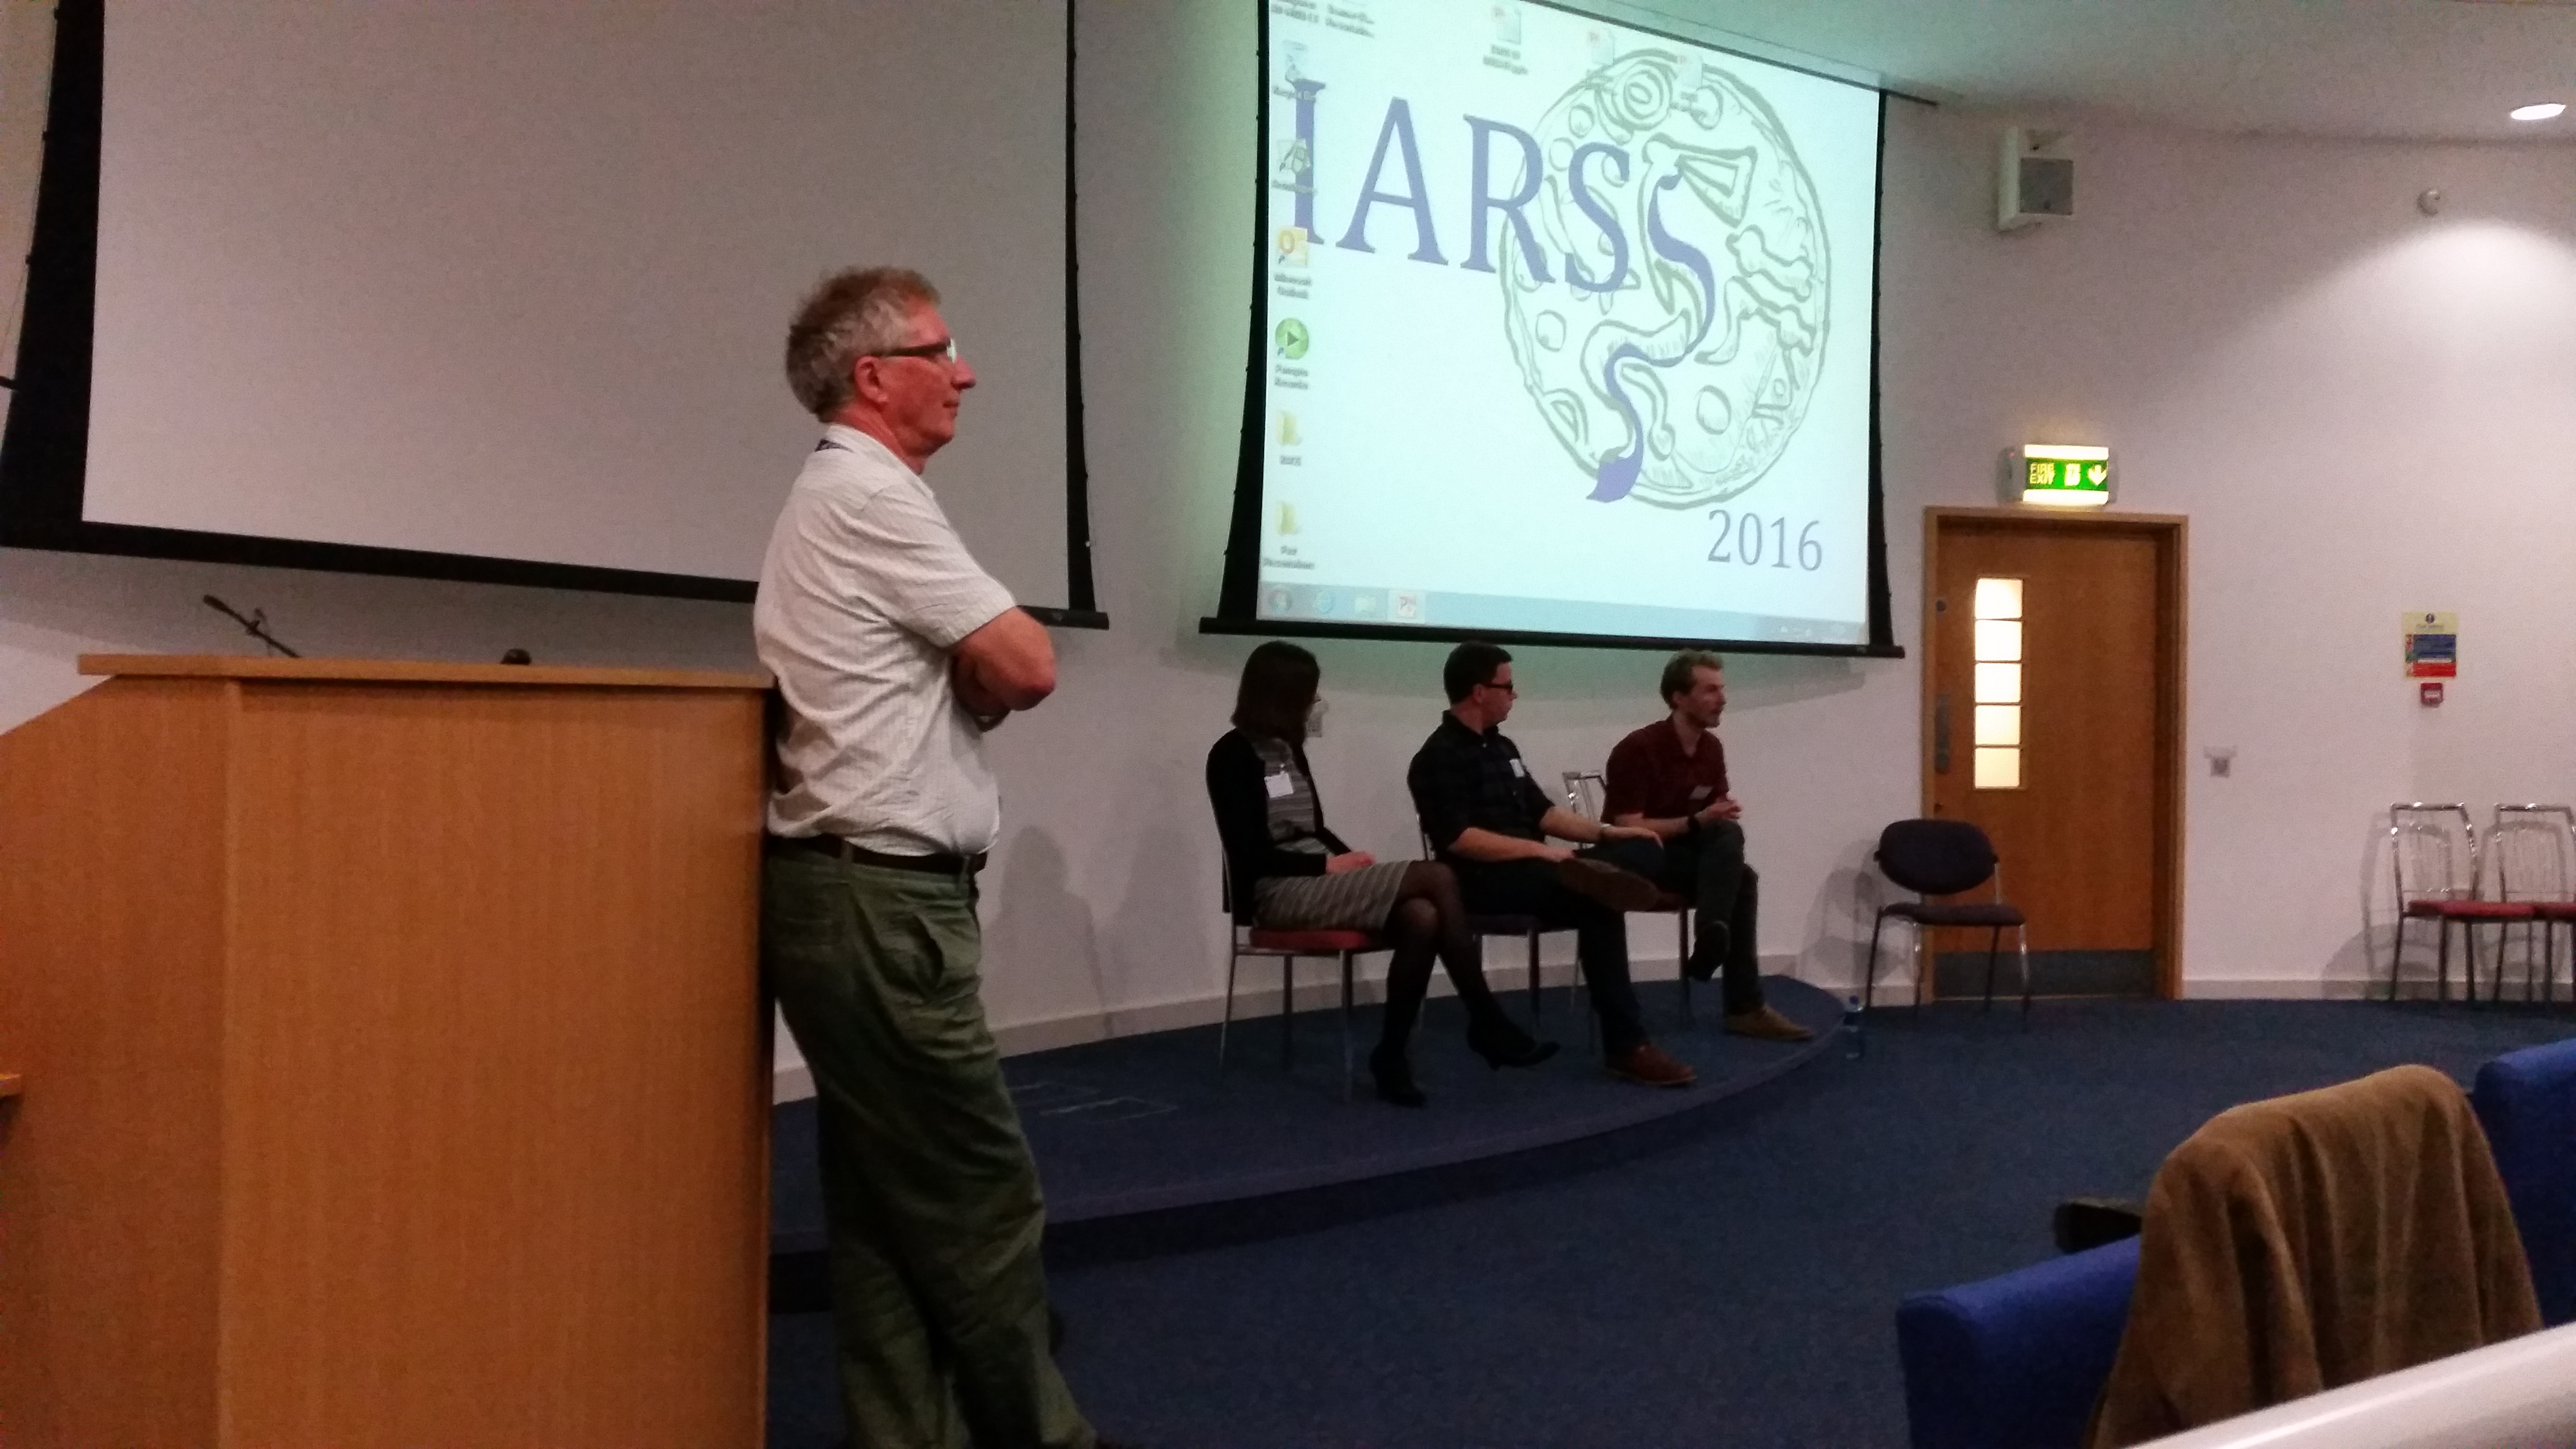
\includegraphics[width=\linewidth]{figures/IARSS_Session}
\caption{<<Description of the figure>>}
\source{<<picture taken by whom?>>}
\label{fig:IARSS_Session}
\end{wrapfigure} 

%\vspace*{2em}

IARSS 2016 was delivered over a two day period, with oral presentations divided into eight sessions, with an additional session for poster presentations. Following a keynote address on the Thursday evening by Prof Colin Haselgrove, University of Leicester, in which he discussed his excavations and ongoing research at the Iron Age site of Stanwick, Yorkshire, sessions began on Friday. The Archaeology of Death, chaired by Dr Andrew Fitzpatrick, began the symposium, with topics ranging from La Tène period burials in the Champagne region, to Early Iron Age cremations in the Adriatic. 
This was followed by Dr Adrian Chadwick, University of Leicester, chairing a session on GIS and landscape archaeology. The session offered interesting insights into the landscapes of north west England and Hungary generated much discussion. Human relationships with the environment were the topic of the penultimate session, chaired by Dr David Smith from the University of Birmingham. Papers ranged in focus from the study of Iron Age chickens, itself part of a study shared across several UK universities, to as far south as the coast of Nigeria. Prof Colin Haselgrove subsequently chaired the Technology session, which included, among other thought provoking papers, the first research to consider what fingerprints might tell us about the age of peoples involved in prehistoric communities.

\begin{wrapfigure}{O}[.3\textwidth]{0.7\linewidth}
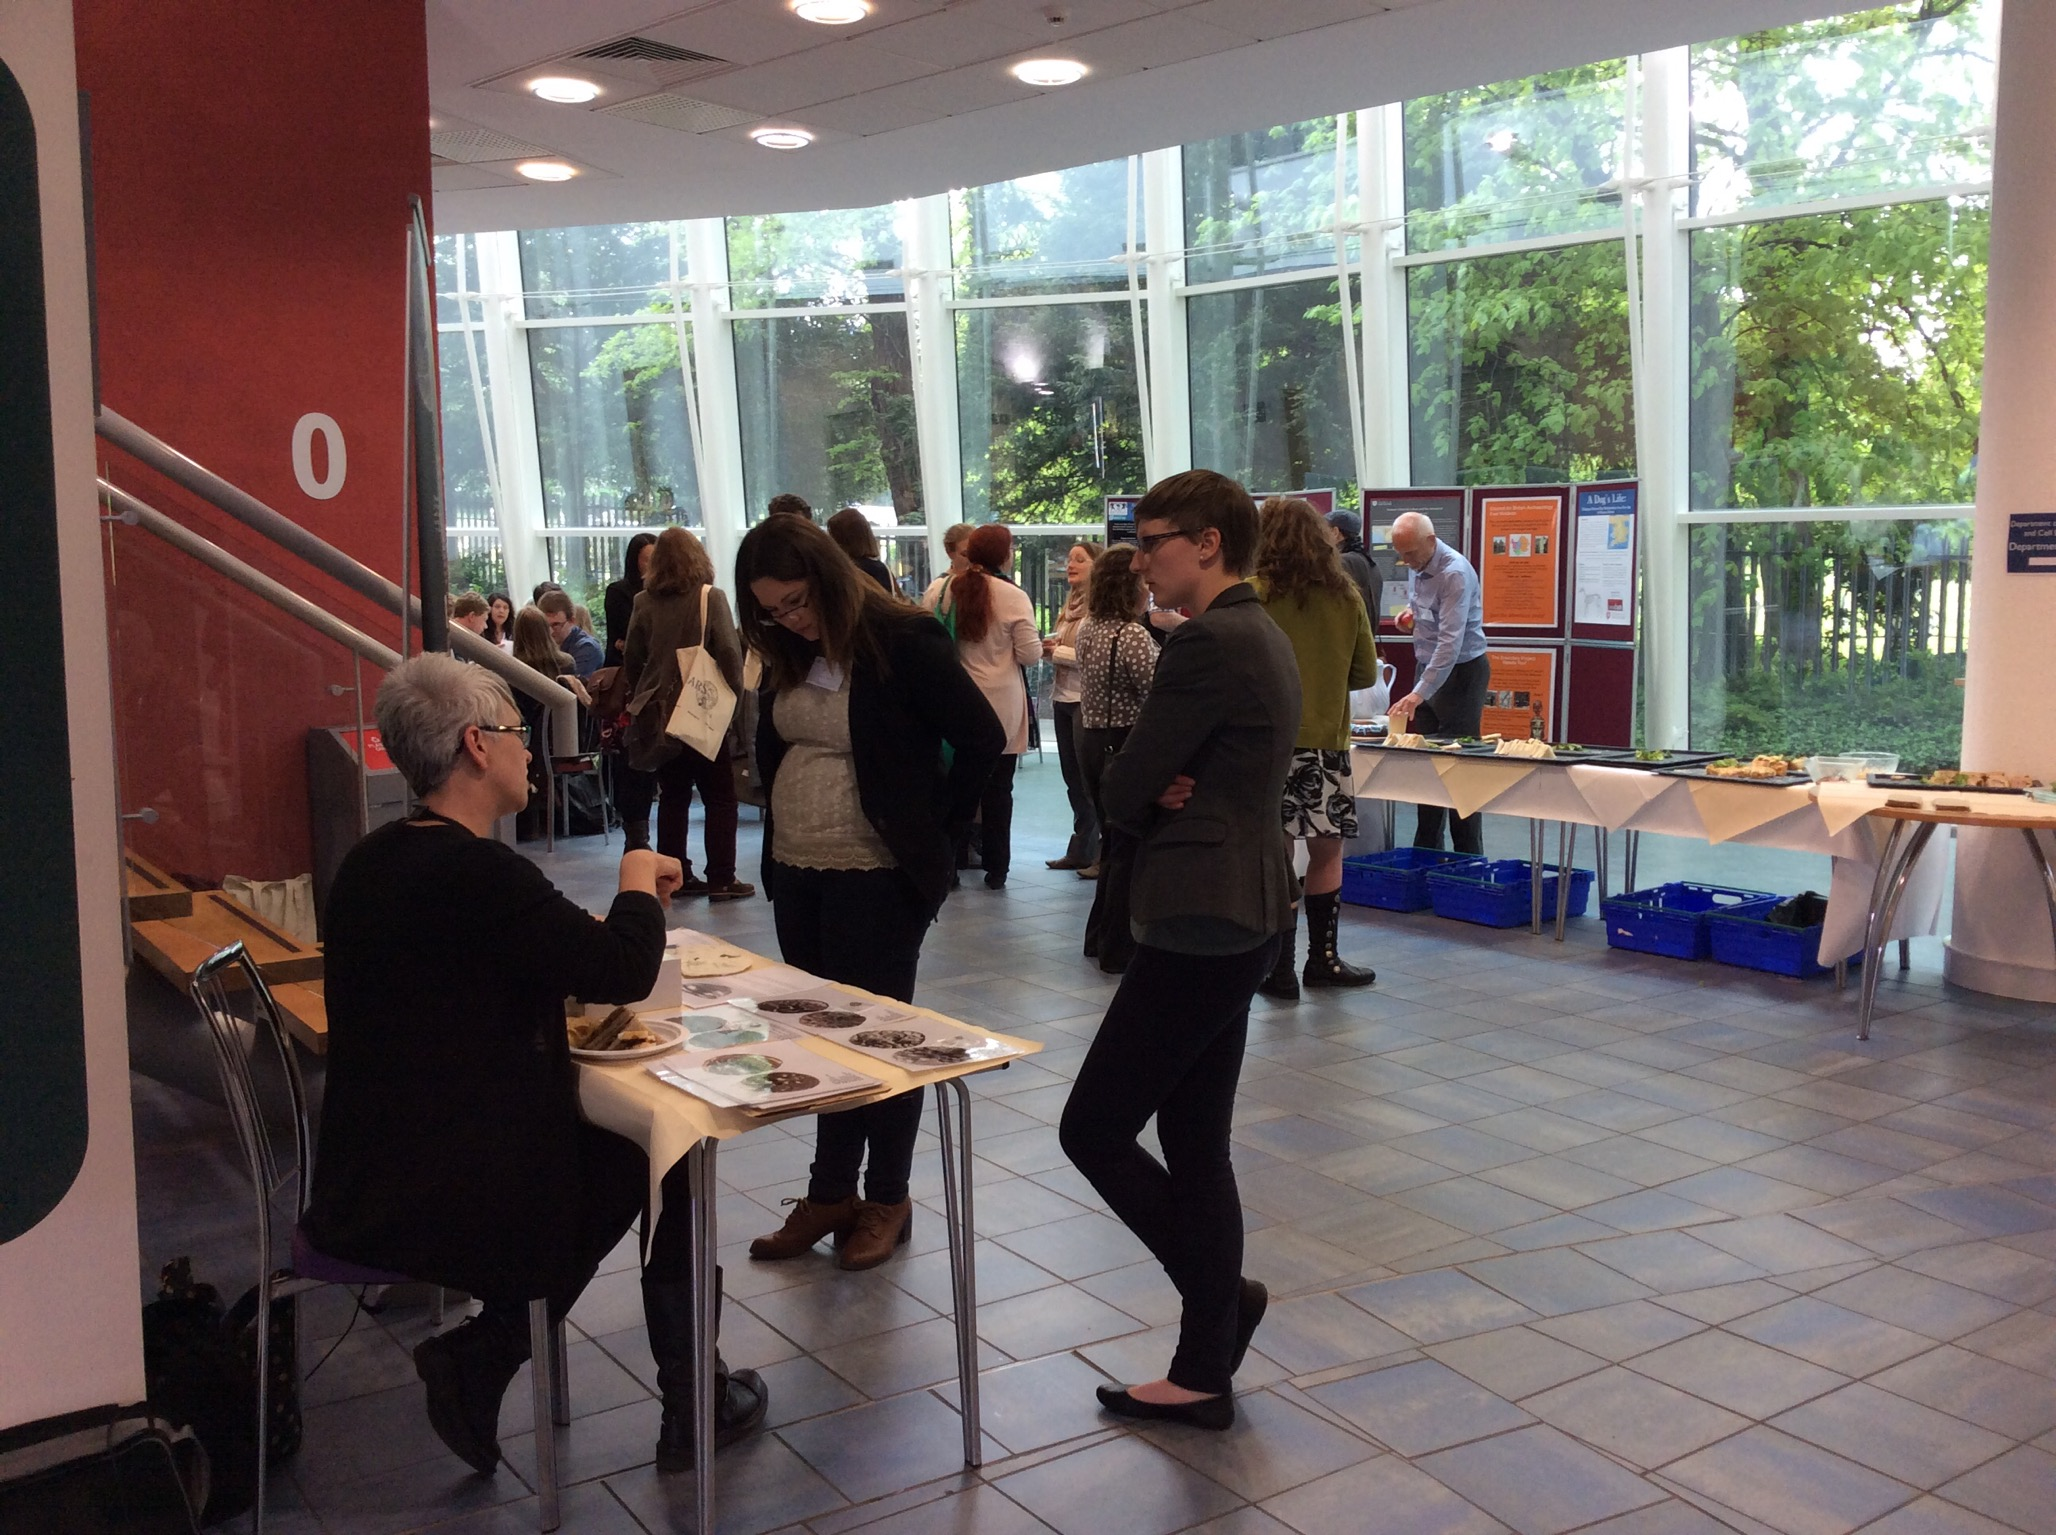
\includegraphics[width=\linewidth]{figures/IARSS_Break2}
\caption{<<Description of the figure>>}
\source{<<picture taken by whom?>>}
\label{fig:IARSS_Break2}
\end{wrapfigure} 
Saturday commenced with Dr Martin Schönfelder of the \foreignlanguage{ngerman}{Römisch\--German\-isches Zentralmuseum --
 Forschungsinstitut für Archäologie} (RZGM), Mainz (GER), chairing two sessions: firstly Hierarchies in
  Society/Settlement and the subsequent Oppida session. Papers in these sessions were highly varied in
   their scope, including historiographical research which considered how French scholars have envisaged
    the Gallic family, and the damage sustained by the Iron Age settlement of Manching during the Second World War. 
Dr~Julia Farley, Curator of European Iron Age Collections at the British Museum, chaired the first of two afternoon sessions about Metalwork (production).  Papers in this session considered issues of object biographies, the Late Bronze-Early Iron Age transition, and the production of metal in Scandinavia. The final session, Metalwork (deposition) considered what we might learn from the placement of metalwork in the landscape, including its colour and composition, and was chaired by Dr~Natasha Hutcheson. 
Dr~Julia Farley returned to deliver the closing address, thereby marking the end of IARSS 2016.

\begin{wrapfigure}{O}[.3\textwidth]{0.7\linewidth}
%\begin{figure*}[!htb]
%\centering
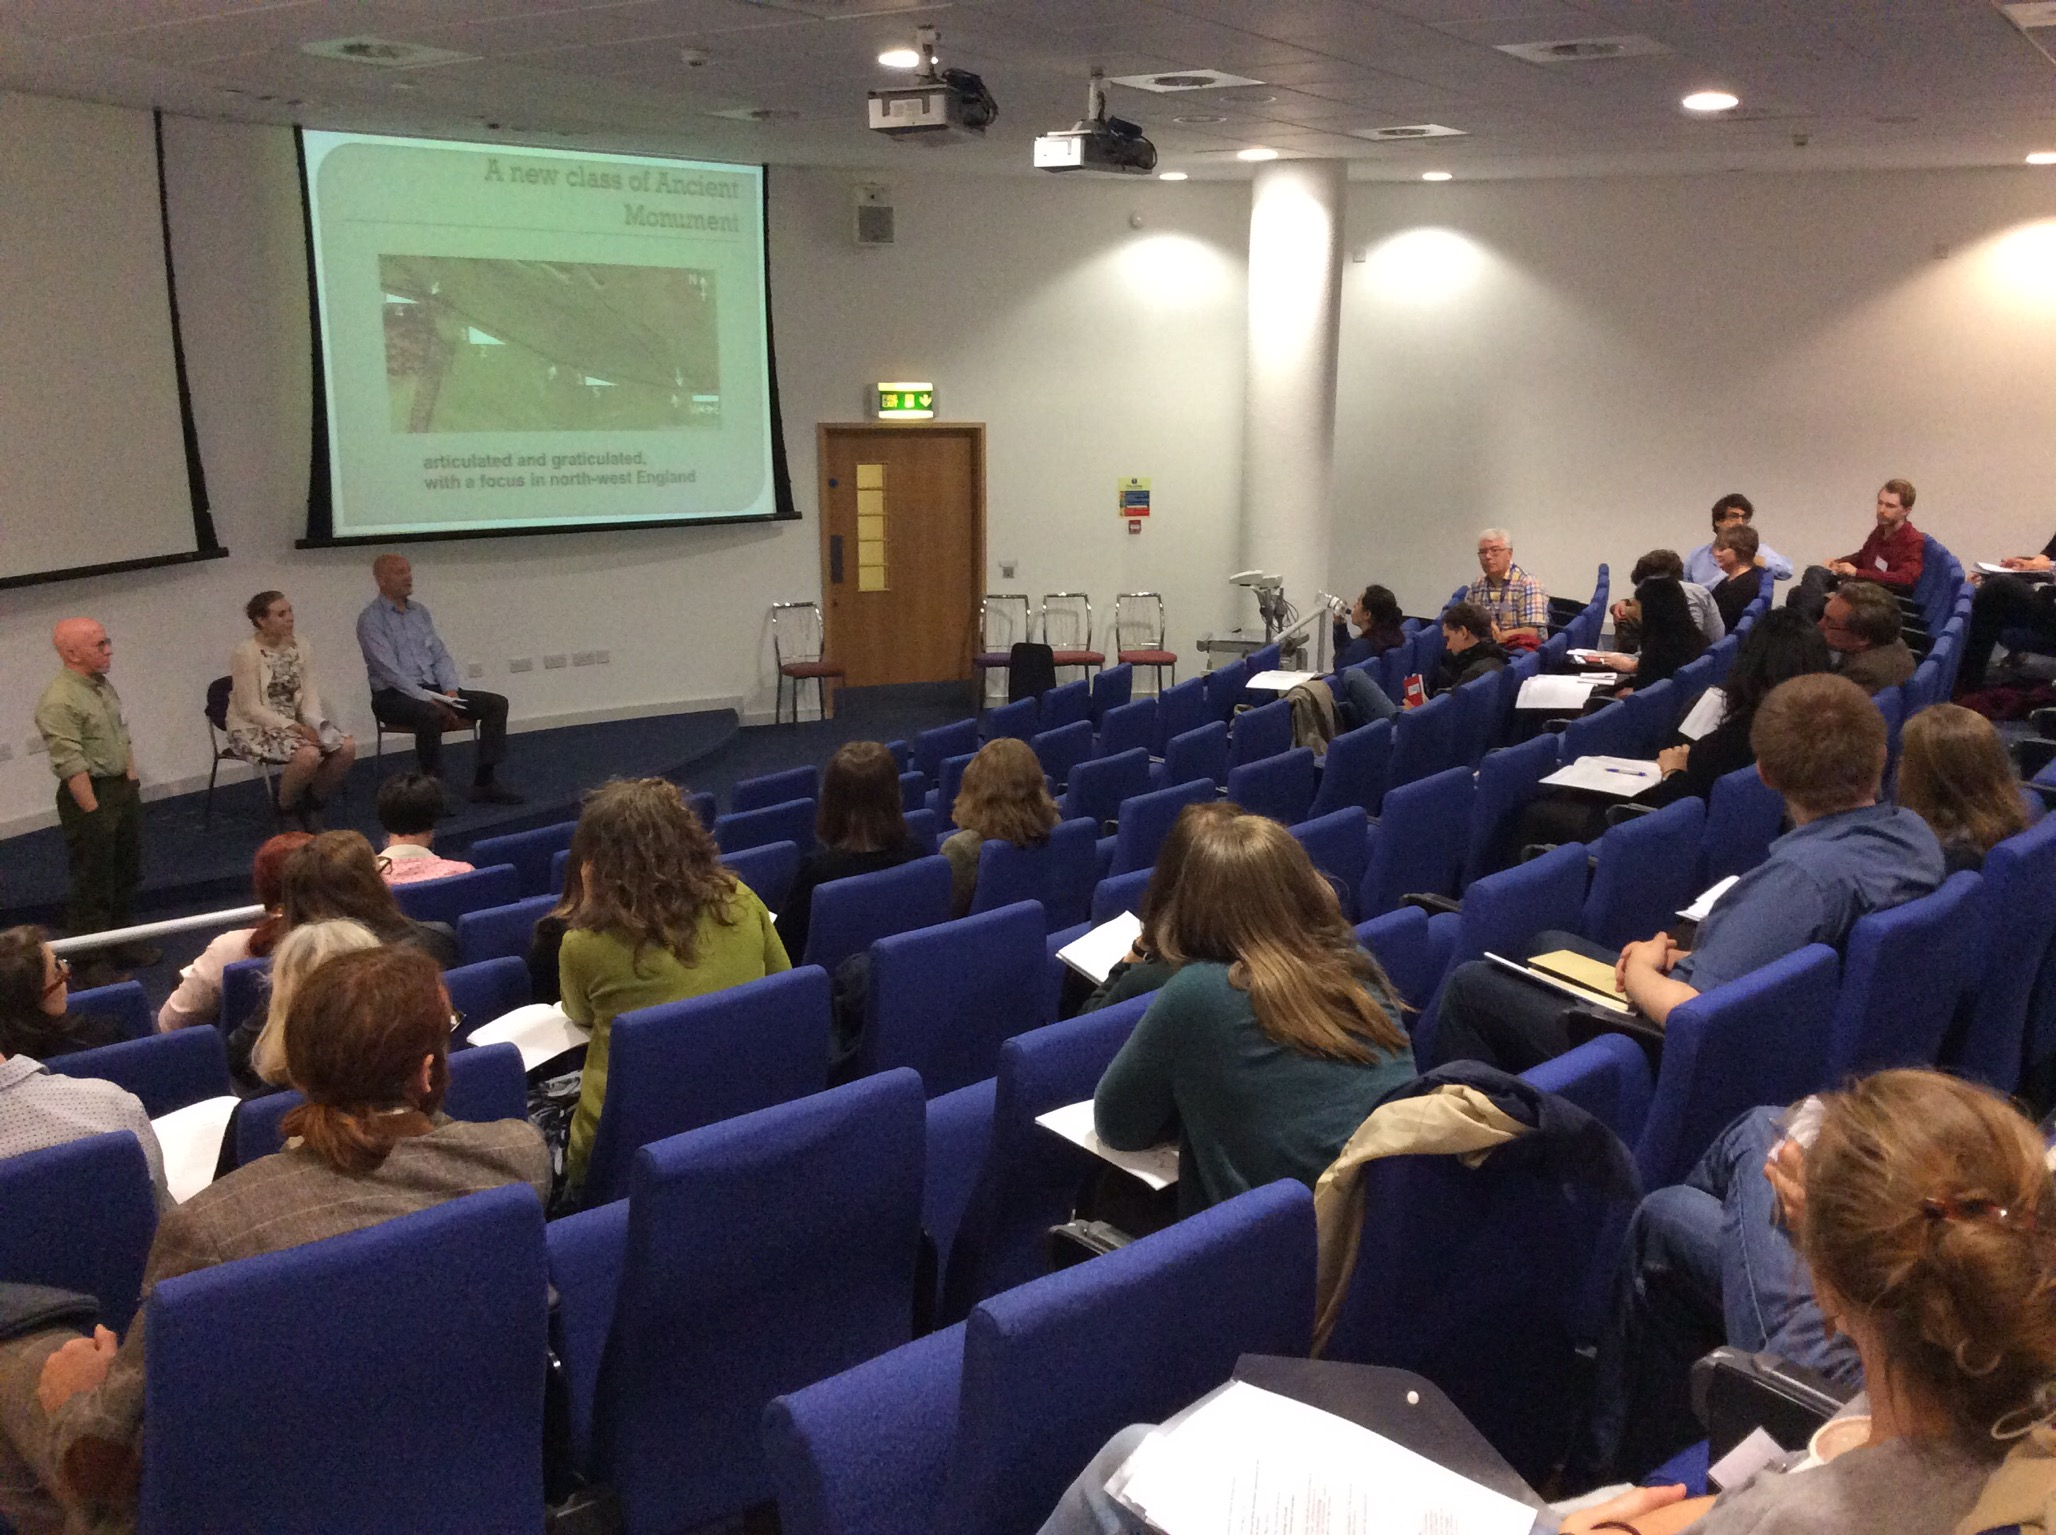
\includegraphics[width=\linewidth]{figures/IARSS_Conference3}
\caption{<<Description of the figure>>}
\source{<<picture taken by whom?>>}
\label{fig:IARSS_Conference3}
%\end{figure*}
\end{wrapfigure} 
IARSS 2016 was warmly received by the majority who attended it, with initial results from an appraisal survey distributed to delegates generating highly positive feedback. In particular this year’s symposium succeeded in being the most international IARSS yet held. 
Of the 53 delegates in attendance, one in five came from continental institutions, whilst of the 27 papers presented, 40 percent were either continental or international in scope. With Dr Martin Schönfelder the organising team succeeded in attracting a European Iron Age specialist, whose research projects range from France via Italy to Poland, as chair, thereby enabling early career researchers to present their studies to an international audience. Although a location for the 20th IARSS has yet to be confirmed, there are hopes that this success in attracting international delegates will result in IARSS 2017 being held at a continental institution. One of the aims of the first IARSS was to broaden the base of Iron Age studies and involve a wide range of individuals and interests from within British Archaeology. 
That IARSS has reached the point where it may become an internationally hosted conference, is a measure of how far this series has come.

%\begin{wrapfigure}{O}[.3\textwidth]{0.7\linewidth}
\begin{figure}[!b]
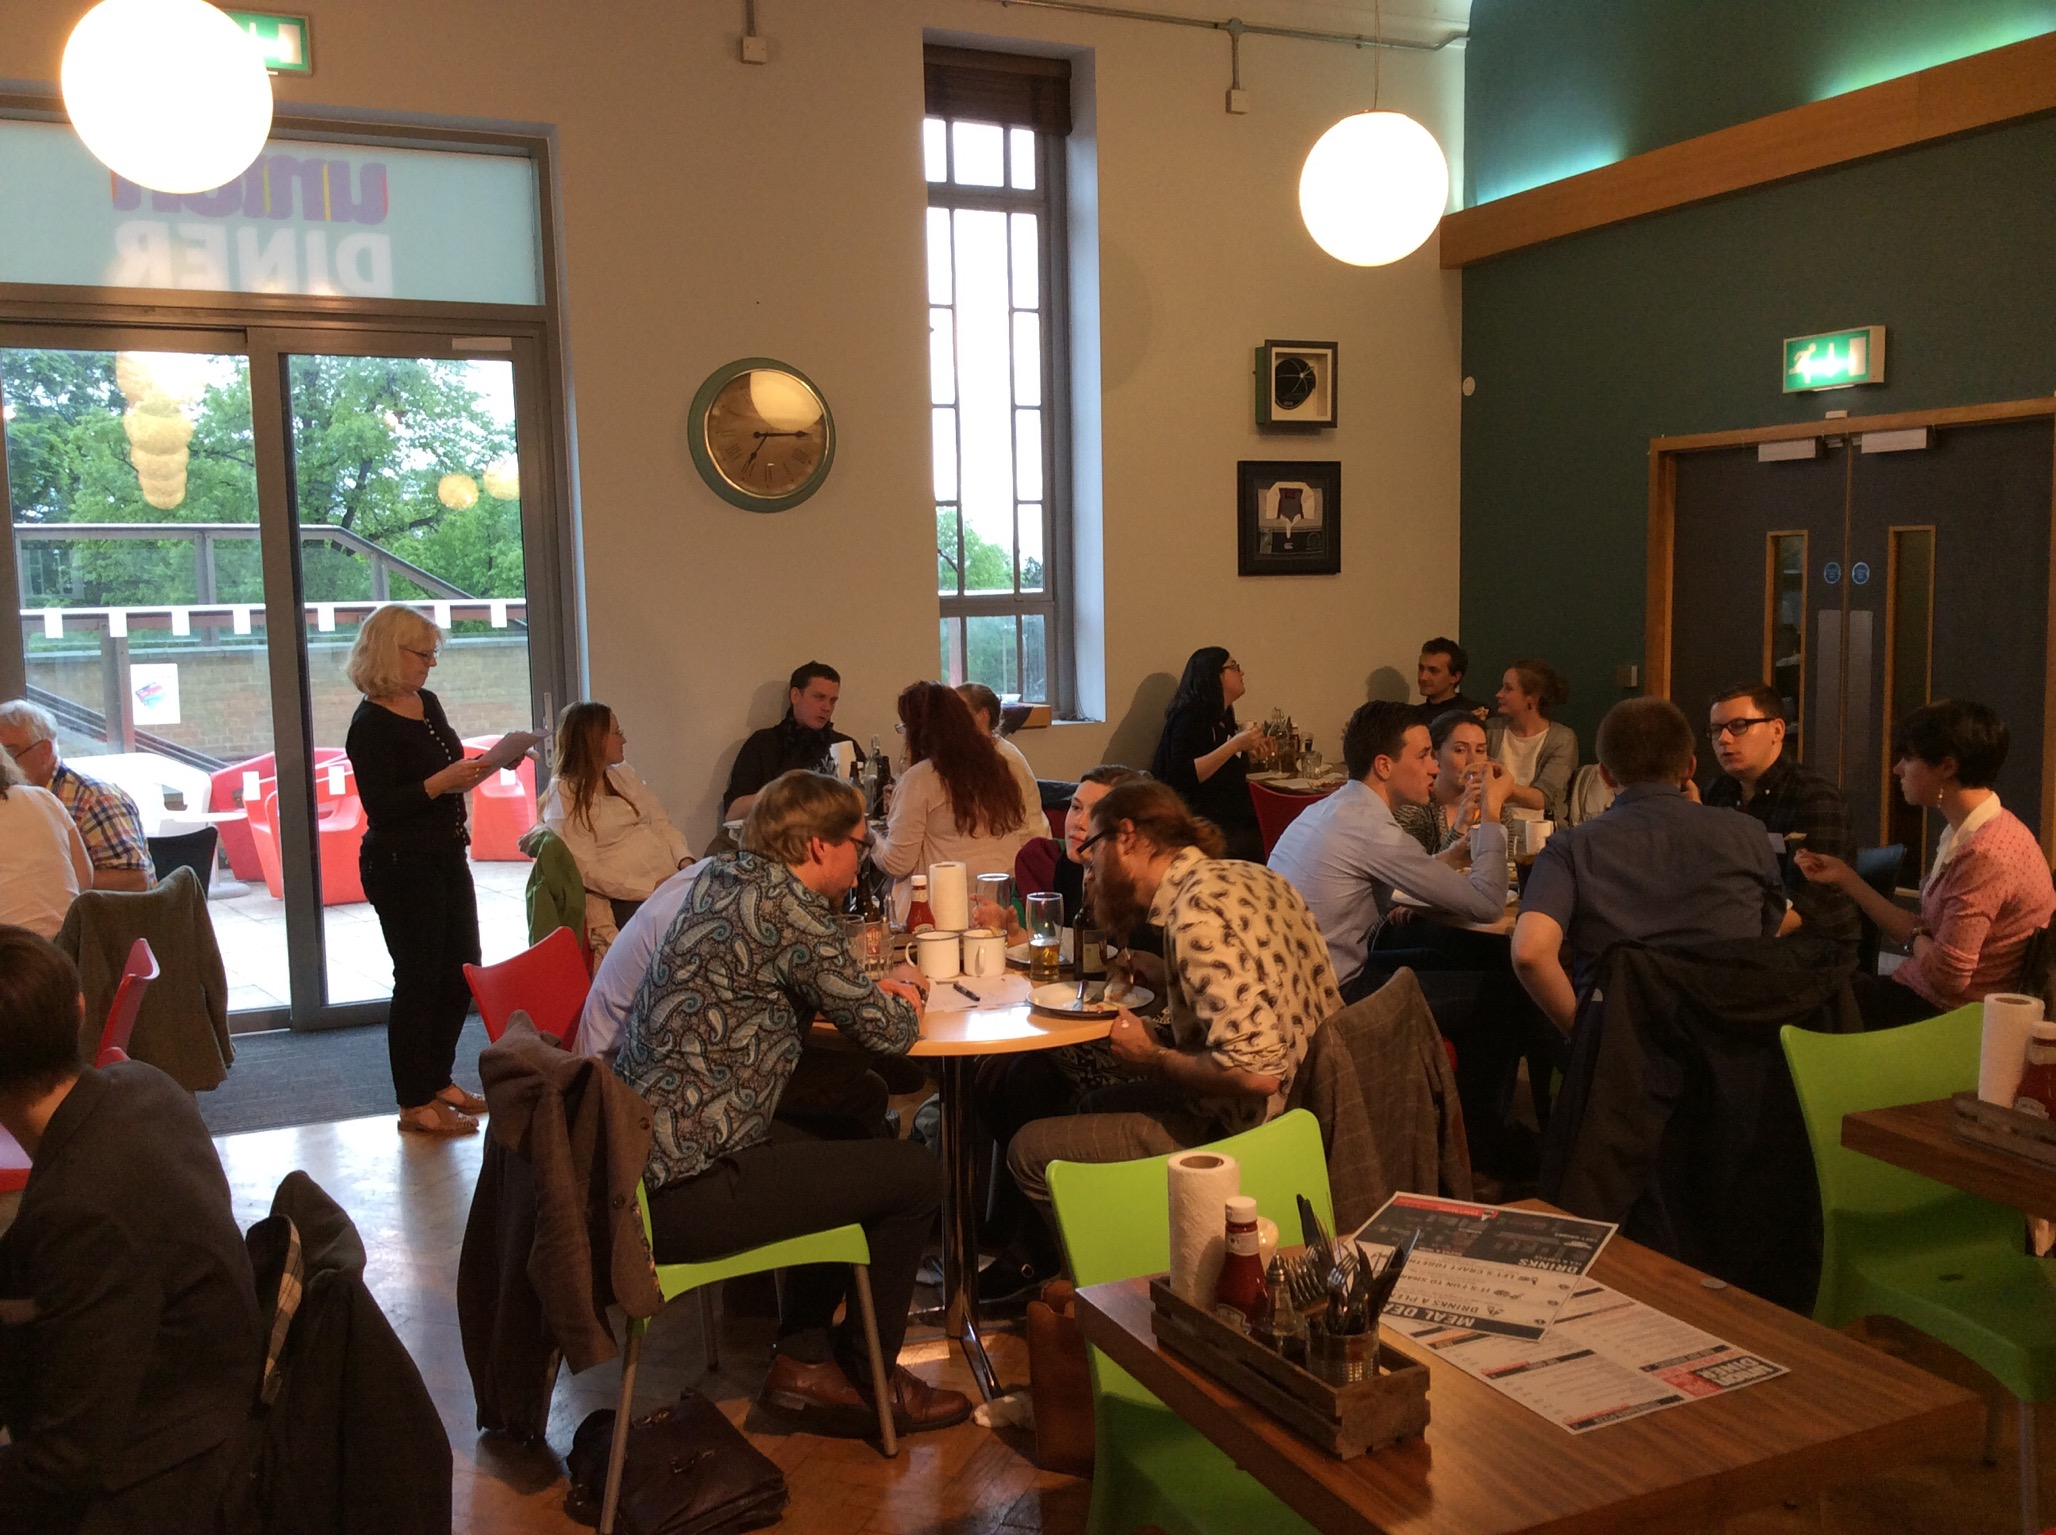
\includegraphics[width=\linewidth]{figures/IARSS_Quiz}
\caption{<<Description of the figure>>}
\source{<<picture taken by whom?>>}
\label{fig:IARSS_Quiz}
\end{figure} 
IARSS 2016 was made possible by the generous contributions of the Prehistoric Society, sponsor of the opening wine reception, 
RGZM, 
sponsor of the internationally chaired sessions on Saturday morning, 
Beta Analytic Radiocarbon Dating, Historic England, the Scottish Archaeological Research Framework and the Later Prehistoric Finds Group. 
In contrast to preceding IARSS events, where delegates were treated to a field trip to a local archaeological site, this year a more ambitious ‘alternative field trip’ was arranged, consisting of nine workshops designed around ‘Routes to a career within heritage and archaeology’. 
Held on Sunday \nth{22} May at the University of Nottingham Museum, the event was sponsored by the Midlands3Cities Doctoral Training Partnership. 
During the day, attendees (which included IARSS delegates as well as researchers from across the UK and with various backgrounds in the Arts and Humanities) were able to select from a variety of workshops, chaired by leading experts in their field. These ranged from 3D modelling and research management, to outreach, heritage practice and working in a museum, with the latter workshop being led by Dr Julia Farley, curator of the critically acclaimed recent \enquote{Celts} exhibition at the British Museum.

The organisers would like to thank their sponsors, including also the University of Leicester Graduate School and College for Social Sciences, Arts and Humanities, the University of Nottingham School of Humanities and the University of Birmingham, for their financial contributions and the University of Leicester School of Archaeology and Ancient History and university staff members for their invaluable support. 



\IJSRAclosing%<<<< DO NOT change this line
\end{document}